%%%%%%%%%%%%%%%%%%%%%%%%%%%%%%%%%%%%%%%%%
% Dreuw & Deselaer's Poster
% LaTeX Template
% Version 1.0 (11/04/13)
%
% Created by:
% Philippe Dreuw and Thomas Deselaers
% http://www-i6.informatik.rwth-aachen.de/~dreuw/latexbeamerposter.php
%
% This template has been downloaded from:
% http://www.LaTeXTemplates.com
%
% License:
% CC BY-NC-SA 3.0 (http://creativecommons.org/licenses/by-nc-sa/3.0/)
%
%%%%%%%%%%%%%%%%%%%%%%%%%%%%%%%%%%%%%%%%%

%----------------------------------------------------------------------------------------
%	PACKAGES AND OTHER DOCUMENT CONFIGURATIONS
%----------------------------------------------------------------------------------------


\documentclass[final,hyperref={pdfpagelabels=false}]{beamer}

\usepackage[orientation=portrait,size=a0,scale=1.6]{beamerposter} % Use the beamerposter package for laying out the poster with a portrait orientation and an a0 paper size

\usetheme{I6pd2} % Use the I6pd2 theme supplied with this template

\usepackage[english]{babel} % English language/hyphenation

\usepackage{amsmath,amsthm,amssymb,latexsym} % For including math equations, theorems, symbols, etc

%\usepackage{times}\usefonttheme{professionalfonts}  % Uncomment to use Times as the main font
%\usefonttheme[onlymath]{serif} % Uncomment to use a Serif font within math environments

\boldmath % Use bold for everything within the math environment

\usepackage{booktabs} % Top and bottom rules for tables
\usepackage{ragged2e}

\graphicspath{{figures/}} % Location of the graphics files

\usecaptiontemplate{\small\structure{\insertcaptionname~\insertcaptionnumber: }\insertcaption} % A fix for figure numbering

%----------------------------------------------------------------------------------------
%	TITLE SECTION 
%----------------------------------------------------------------------------------------

\title{\Huge Pluie de Coke sur Tokyo} % Poster title

\author{Valentin Baillard, Alexandre Goy et Nicolas Vasselin} % Author(s)

\institute{Fili\`ere M\'etiers de la Recherche, CentraleSup\'elec, sous la supervision de Cristina Maniu} % Institution(s)

%----------------------------------------------------------------------------------------
%	FOOTER TEXT
%----------------------------------------------------------------------------------------

\newcommand{\leftfoot}{} % Left footer text

\newcommand{\rightfoot}{valentin.baillard@student.ecp.fr \\ alexandre.goy@student.ecp.fr \\ nicolas.vasselin@student.ecp.fr} % Right footer text


%----------------------------------------------------------------------------------------

\begin{document}

\addtobeamertemplate{block end}{}{\vspace*{2ex}} % White space under blocks

\begin{frame}[t] % The whole poster is enclosed in one beamer frame

\begin{columns}[t] % The whole poster consists of two major columns, each of which can be subdivided further with another \begin{columns} block - the [t] argument aligns each column's content to the top

\begin{column}{.02\textwidth}\end{column} % Empty spacer column

\begin{column}{.465\textwidth} % The first column

%----------------------------------------------------------------------------------------
%	CONTEXTE
%----------------------------------------------------------------------------------------
            
\begin{block}{{\Large Contexte}}

Imaginons que dans le ciel de Tokyo volent deux types de drones.\\
\begin{itemize}
\item Drones yakuzas
\begin{itemize}
\item \textit{Objectif} : livrer de la coca\"{i}ne \`a certains points strat\'egiques
\item \textit{Contraintes} : \'eviter les policiers et les collisions
\end{itemize}
\item Drones policiers
\begin{itemize}
\item \textit{Objectif} : capturer les yakuzas
\item \textit{Contraintes} : \'eviter les collisions
\end{itemize}
\end{itemize} \mbox{} \\
{\large \textbf{Objectifs de l'\'etude}} \\
\begin{itemize}
\item Bien poser le probl\`eme : 
\begin{itemize}
\item Qu'est-ce qu'un comportement de groupe ? Que mesurer ?
\item Qu'est-ce qu'une strat\'egie optimale ? Que maximiser ?
\end{itemize}
\item Montrer que des comportements de groupe \'emergent dans les strat\'egies optimales
\end{itemize}
\end{block}

%----------------------------------------------------------------------------------------
%	SIMULATIONS
%----------------------------------------------------------------------------------------

\begin{block}{{\Large Premi\`eres simulations}}
\begin{figure}[h!]
   \begin{minipage}[b]{0.50\linewidth}
      \centering 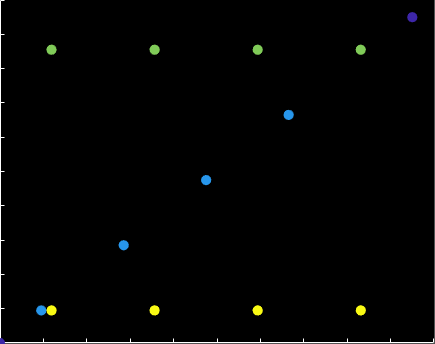
\includegraphics[scale=1.4]{simu_0.png}
      \caption{\text{ }$0$ it\'erations}
   \end{minipage}\hfill
   \begin{minipage}[b]{0.50\linewidth}   
      \centering 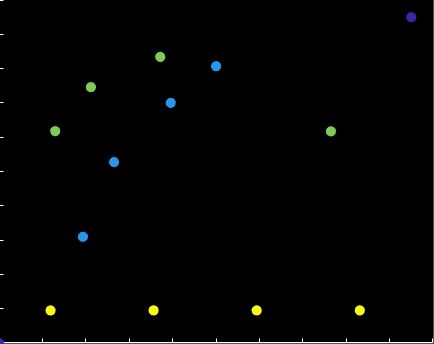
\includegraphics[scale=1.4]{simu_100.png}
      \caption{\text{ } $100$ it\'erations}
   \end{minipage}
   \begin{minipage}[b]{0.50\linewidth}
      \centering 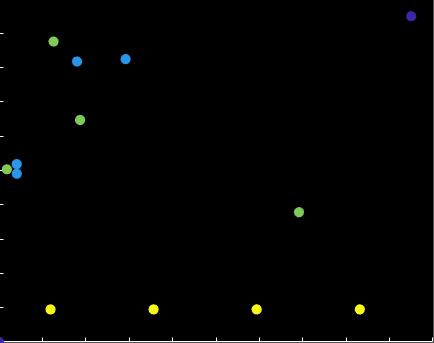
\includegraphics[scale=1.4]{simu_200.png}
      \caption{\text{ } $200$ it\'erations}      
   \end{minipage}\hfill
   \begin{minipage}[b]{0.50\linewidth}   
      \centering 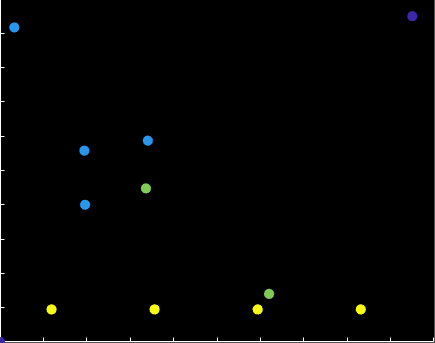
\includegraphics[scale=1.4]{simu_300.png}
      \caption{\text{ } $300$ it\'erations}      
   \end{minipage}
   \begin{minipage}[b]{0.50\linewidth}
      \centering 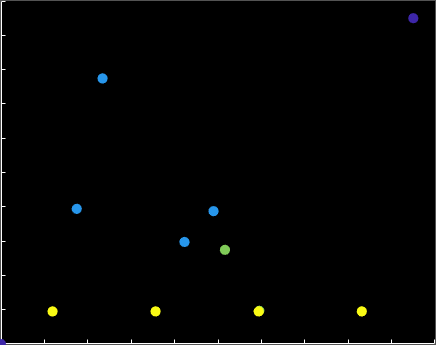
\includegraphics[scale=1.4]{simu_400.png}
      \caption{\text{ } $400$ it\'erations}
   \end{minipage}\hfill
   \begin{minipage}[b]{0.50\linewidth}   
      \centering 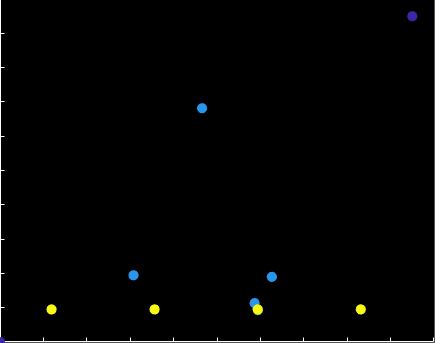
\includegraphics[scale=1.4]{simu_500.png}
      \caption{\text{ } $500$ it\'erations}
   \end{minipage}
   
\end{figure}

\end{block}

%----------------------------------------------------------------------------------------

\end{column} % End of the first column

\begin{column}{.03\textwidth}\end{column} % Empty spacer column
 
\begin{column}{.465\textwidth} % The second column

%----------------------------------------------------------------------------------------
%	MATHEMATICAL SECTION
%----------------------------------------------------------------------------------------

\begin{block}{{\Large Approche par potentiels}}

\begin{itemize}
\item Potentiel du point de vue d'un policier $\overline{p}$ :
\begin{align*}
U_{\overline{p}} = \sum_{y \in Y} U_{\to y} + \sum_{p \in P\setminus\{\overline{p}\}} U_{\gets p} + U_{\gets E}
\end{align*}
\item Potentiel du point de vue d'un yakuza $\overline{y}$ :
\begin{align*}
V_{\overline{y}} = V_{\to O} + \sum_{y \in Y \setminus \{\overline{y}\}} V_{\gets y} + \sum_{p \in P} V_{\gets p} + V_{\gets E}
\end{align*}
\item D\'eplacement dans la direction du gradient de son potentiel
\item Vitesse born\'ee
\end{itemize}
\end{block}
\begin{figure}
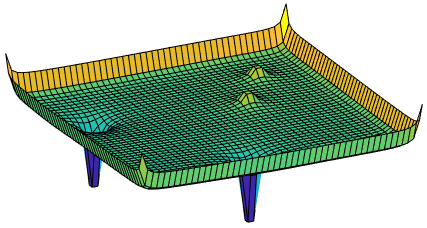
\includegraphics[width=0.8\linewidth]{potentials.png}
\caption{\text{ } Potentiel d'un policier (pics = autres policiers, puits = yakuzas)}
\end{figure}

%----------------------------------------------------------------------------------------
%	TO BE CONTINUED
%----------------------------------------------------------------------------------------
{
\setbeamercolor{normal text}{fg=black, bg=white}
\setbeamercolor{block body}{bg=dirtlight,fg=black}
\setbeamercolor{block title}{fg=black,bg=dirt}
\setbeamercolor{structure}{fg=dirtdark}
\begin{block}{{\Large Approche originale}}



\begin{itemize}
\item Potentiels $\sim$ champ \'electrique $\to$ ajout d'un champ magn\'etique
\begin{itemize}
\item \textit{Objectif} : permettre des man\oe uvres de contournement
\item \textit{Approche} : physique des plasmas
\end{itemize}
\item Choix des param\`etres
\begin{itemize}
\item \textit{Objectif} : trouver les strat\'egies optimales
\item \textit{Approche} : apprentissage adversorial
\end{itemize}
\end{itemize}

\end{block}
}

%----------------------------------------------------------------------------------------
%	REFERENCES
%----------------------------------------------------------------------------------------

\begin{block}{{\Large R\'ef\'erences}}
Merci \`a Cristina Maniu qui nous a efficacement supervis\'es. Merci \'egalement \`a Matlab.
%\nocite{*} % Insert publications even if they are not cited in the poster
%\small{\bibliographystyle{unsrt}
%\bibliography{sample}}

\end{block}

%----------------------------------------------------------------------------------------

\end{column} % End of the second column

\begin{column}{.015\textwidth}\end{column} % Empty spacer column

\end{columns} % End of all the columns in the poster

\end{frame} % End of the enclosing frame

\end{document}

